\chapter{Local coherence and block decomposition}
\label{ch:p2:lc}

\dictum[Unknown]{%
  Teach your algorithm physics and it will perform better.}%
\vskip 1em

\readit{2}

\worktodo{
* local coherence
	* Local coherence
	* block decomp -> subspace deflation with non-trivial lattice index
}

% \worktodo{
% * LMA -> as subspace deflation
% 	* eg: 2pt corr estimator -> its prop decomp, [Q,P]=0 <=> phi = modes of Q
% 	* extensions to LMA
% 		* AMA with its prop decomp
% 	* problems -> volume scaling, expensive modes, memory, ...
% 		* X-term problem
% 		* V2 problem
% }

\tldr{lc intro}
In the last chapter, we have introduced a subspace with spinors and operators acting on it.
We did not yet take an attempt to interpret its structure.
In this chapter, with the concept of local coherence of low quark modes~\cite{Luescher2007}, also known as weak approximation property~\cite{Babich:2010qb} we will change that by introducing a coarse lattice.
Referring to operators restricted to these subspaces as \emph{coarse} operators will then be manifest.

\tldr{free theory low modes and staircase functions}
In momentum space, the low modes of the Dirac operator in the free quark theory are sharp delta functions at small momenta $\lvert p \rvert$ making them smooth, slowly oscillating plane waves in position space $x$, whose amplitude only depends on $p$ and is spread over the whole lattice.
A good approximation for them in position space are constant spinor fields.
In order to include the slow oscillations, we may project these fields to a block decomposition of the lattice whose block size catches well the resolution of the wave, see \cref{fig:free:theory}.
\begin{figure}
    \centering
    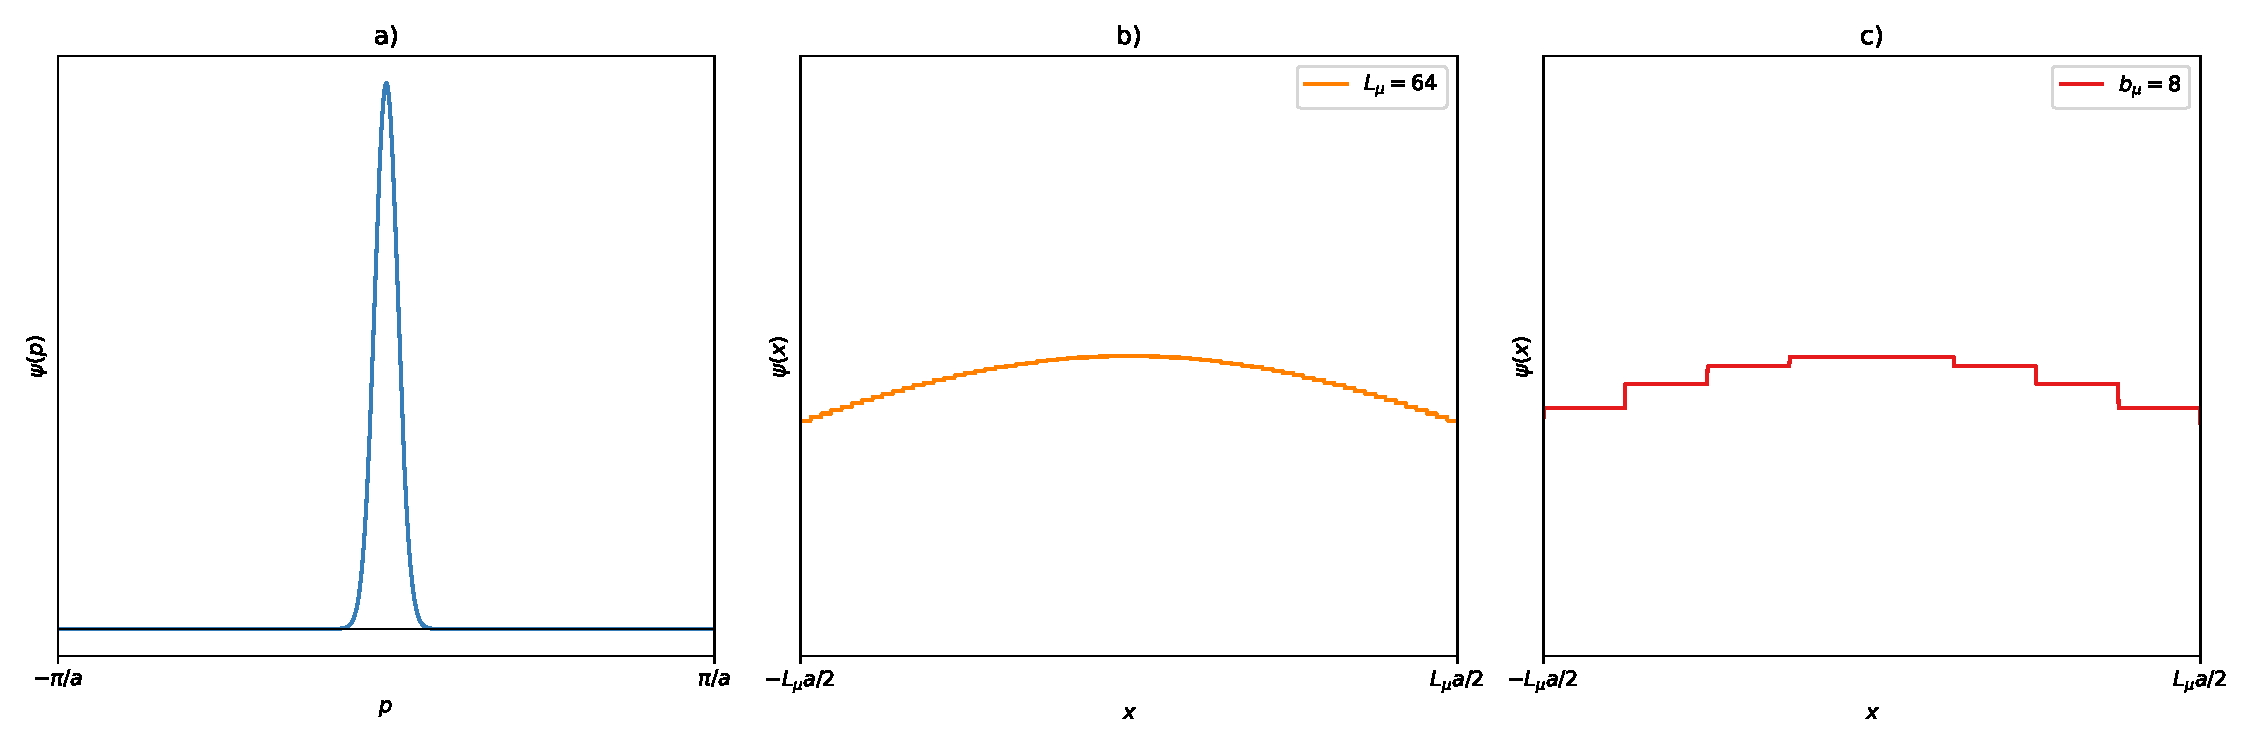
\includegraphics[width=\linewidth]{\dir/img/free_theory}
    \caption{Quantitative picture of low modes in the free theory. Panel a) shows the sharp peak in momentum space centered around zero, whereas panel b) shows the same mode in position space on a finite lattice. Panel c) shows the approximation when using constant modes projected to blocks. The fact that the low modes are flat in position space makes the approximation suitable.}
    \label{fig:free:theory}
\end{figure}
The actual modes can then be approximated by staircase-shaped functions constant on each block.
The smaller the block size, the smoother the approximation, and in the limit of the block size approaching the lattice spacing $a$ on all \num{4} extents, we retain the exact form of the modes on the lattice.

\tldr{lc definition}
These considerations certainly hold in the free theory, but in the interacting theory with dynamic gauge fields the situation looks different.
Inspired by the free theory, the property of local coherence of some linear independent set of fields $\mathcal{M}$, states that these fields are to a good approximation contained in the span of another (possibly larger) set of fields $\Pi(\mathcal{B})$ generated by block projecting a small bootstrap set $\mathcal{B} \subset \mathcal{M}$, symbolically
\begin{equation} \label{eq:local:coherence:sets}
\lvert \mathcal{B} \rvert \ll \lvert \Pi(\mathcal{B}) \rvert \;,
\qquad
\mathcal{B} \xrightarrow[\text{projection}]{\text{block}} \Pi(\mathcal{B}) \;,
\qquad
\vslattice_{\mathcal{B}} \subset \vslattice_{\Pi(\mathcal{B})} \;,
\end{equation}
where $\vslattice_{\mathcal{A}}$ is the vector space generated by the span of the vectors $\mathcal{A}$, $\vslattice_{\mathcal{A}} = \vspan{\mathcal{A}}$.
The key equation describing the property is that
\begin{equation} \label{eq:local:coherence:set:approx}
\vslattice_{\mathcal{M}} \subsetsim \vslattice_{\Pi(\mathcal{B})}
\end{equation}
holds up to small deficits.
Local coherence of low modes means that the $N \gg \coarse{\Nc}$ lowest modes of the Dirac operator can be well represented using a block-projected basis out of the $\coarse{\Nc}$ lowest modes.

\tldr{block projection and coarse lattice}
A few things still need to be formalized for the above procedure, for instance the block projection.
We start by considering a block decomposition of the full spacetime lattice $\idxspacetime$ into $\coarse{V} \in \mathbb{N}$ equally-sized disjoint blocks
\begin{equation} \label{eq:coarse:lattice}
\idxspacetime
= \{ (x_0,x_1,x_2,x_3) \mid 0 \leq x_{\mu} < L_{\mu} \}
= \bigcup_{\coarse{y} \in \coarse{\idxspacetime}} B_{\coarse{y}} \;.
% \qquad
% B_{x} \cap B_{y} = \emptyset \;,
% \qquad
% x \neq y \in \coarse{\idxspacetime}\;,
\end{equation}
The block extents are multiples of the lattice extents (no summation over $\mu$)
\begin{equation}
L_{\mu} = b_{\mu} \coarse{L}_{\mu} \;,
\qquad
b_{\mu}, \coarse{L}_{\mu} \in \mathbb{N} \;.
\end{equation}
They are defined to contain the subset of lattice points they cover
\begin{equation}
B_{\coarse{y}} = \{ x \in \idxspacetime \mid x_{\mu} - \coarse{y}_{\mu} b_{\mu} < b_{\mu} \} \;,
\end{equation}
parametrized by their position $\coarse{y}$ in the block grid.
The $\coarse{y}$ are new coarse coordinates in a coarse lattice $\coarse{\idxspacetime}$ with coarse extents $\coarse{L}_{\mu}$ defined analogous to the fine-grid lattice,
\begin{equation}
\coarse{\idxspacetime} = \{ \coarse{y} = (\coarse{y}_0, \coarse{y}_1, \coarse{y}_2, \coarse{y}_3) \mid 0 \leq \coarse{y}_\mu < \coarse{L}_\mu\} \;.
\end{equation}

\tldr{block projection def and gram schmidt reorthonormalization}
The block projection is defined via projectors to the blocks $B_{\coarse{y}}$ acting on spinor fields $\psi$ as
\begin{equation}
P_{\coarse{y}} \fieldx{\psi}{x} =
\begin{cases}
\fieldx{\psi}{x} & \text{if } x \in B_{\coarse{y}} \;, \\
0 & \text{otherwise.}
\end{cases}
\end{equation}
The projected set in \cref{eq:local:coherence:sets} can now be specified as the reorthonormalized projected spinors
\begin{equation}
\Pi(\mathcal{B}) = \gramschmidt{ \{ P_{\coarse{y}}\psi \mid \psi \in \mathcal{B} \; \text{and} \; \coarse{y} \in \coarse{\idxspacetime} \} } \;,
\end{equation}
where $\gramschmidt{\mathcal{A}}$ is the Gram-Schmidt orthonormalized set provided an arbitrary linear independent set $\mathcal{A}$.

\tldr{coarse color, coarse spacetime indices}
This procedure specifies a second coarser lattice $\coarse{\lattice}$ analogue to \cref{sec:lattice:definition} but with different degrees of freedom for spin, color and spacetime.
As of now, we will interpret the field index $\coarse{a}$ in $\psi_{\coarse{a}} \in \mathcal{B}$ for some (arbitrary) enumeration of the fields as coarse color.
This will become clear later.
The block index $\coarse{y} \in \coarse{\idxspacetime}$ is straightforwardly interpreted as coarse spacetime index and finally the coarse spin is trivial for now.
This gives us $(\coarse{N}_s, \coarse{\Nc}) = (1, \lvert \mathcal{B} \rvert)$ as well as a coarse volume as product of the coarse lattice extents and coarse spinors defined on the coarse lattice with coarse internal degrees of freedom given by the coarse spin and colors.

\tldr{deficit}
The quality of the approximation can be quantified with the deficit
\begin{equation}
\epsilon_{\psi} = \frac{\norm{ (1-P) \psi }}{\norm{\psi}} \in [0,1] \;,
\qquad
\psi \in \mathcal{M} \;,
\end{equation}
where $P$ is the Hermitian projector to the block projected subspace,
\begin{equation} \label{eq:lc:projector}
P = \sum_{\phi \in \Pi(\mathcal{B})} \phi \phi^{\dagger} \;.
\end{equation}

\tldr{deficit plotted, we observe lc}
We showcase local coherence of low modes of the Hermitian Dirac operator $Q = \gamma^{5} D$ in \cref{fig:lc}.
\begin{figure}
    \centering
    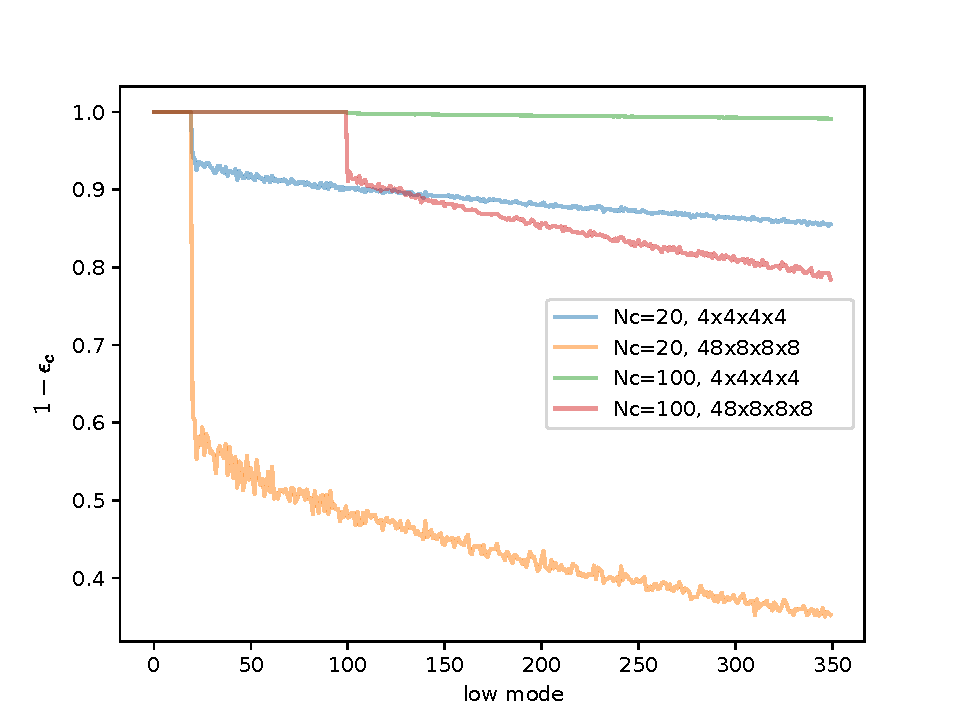
\includegraphics[width=0.7\linewidth]{\dir/img/lc}
    \caption{Local coherence of the low modes of $Q$ tested on ensemble F7 of global lattice size $(L_0,L_1,L_2,L_3) = (96, 48, 48, 48)$, see \cref{tab:mglma:ensembles}. The figure shows the value of $1 - \epsilon_i = \norm{P \evec_i}$ on the y-axis versus the eigenmode number $i$ on the x-axis, where $\evec_i$ is the $i$-th normalized lowest mode for two different values of $\Nc$ and block sizes. \takenfull }
    \label{fig:lc}
\end{figure}
The plot shows the fraction of the \num{350} lowest modes that are contained in the blocked subspace constructed from only the $\coarse{\Nc} = 20, 100$ lowest ones, $\mathcal{B} = \{ \evec_i \mid 0 \leq i < \coarse{\Nc} \}$.
The modes were determined up to relative precision of $\norm{Q \evec - \lambda \evec}/\norm{\evec} \leq 10^{-12}$ for an eigenmode $\evec$ with eigenvalue $\lambda$.
Different number of low modes $\coarse{\Nc}$ and block extents where used for the bootstrap set to generate subspaces of differing sizes.
Block sizes of $b_{\mu} = 4, 8$ correspond to physical extents of $b_{\mu} a \approx $ \u{0.25}{\femto\metre} and $b_{\mu} a \approx $ \u{0.5}{\femto\metre} respectively.
As analytically expected, the spinors in the bootstrap set are represented exactly with no deficit, \ie $1 - \epsilon_i = 1$ for $\psi \in \mathcal{B}$.
Spinors in $\mathcal{M} \setminus \mathcal{B}$ on the other hand have deficits larger than zero, but nevertheless they are well represented.
The effect of a finer block grid or an increase in low modes results in better overlaps as expected.
Even with a very modest number of $\coarse{\Nc}=20$ low modes and a block size of $4^4$, we already contain $85-90\%$ of the $350$ lowest modes.
Notice that for $\coarse{\Nc}=100$ and block size of $4^4$, the dimension $\coarse{d}$ of the coarse-grid operator $\coarse{Q}$ is already $3.2\%$ of the dimension $d$ of the fine-grid Dirac operator $Q$.
%One might be tempted to drive the number of low modes to the extreme, while having very small blocks
%, but the number of blocks has a negative impact on the condition of $\coarse{Q}$.

\tldr{used in inexact deflation and MG algos}
We note that this property has been crucial to create subspaces with very inexact rough low modes to obtain powerful preconditioners for Krylov subspace solvers, called inexact deflation~\cite{Luescher2007} or multigrid~\cite{Babich:2010qb}.
Furthermore, the property has been used to accelerate the Lanczos algorithm to generate low modes~\cite{Clark_2018}.
The extension of what will follow to using modes determined with a low accuracy is straightforward as we will not assume any special properties of the fields in the bootstrap set.

\tldr{LMA as trivial blocking}
Finally we briefly revisit low-mode averaging one more time to show that it is a pathological case of the above.
The projector $P$ used in low-mode averaging, see \cref{eq:lma:projector}, can be obtained by a block extent equal to the fine-grid lattice extent of $b_{\mu} = L_{\mu}$, \ie one big block covering the whole lattice, making the coarse lattice trivial with a volume $\coarse{V} = 1$.
It leaves only non-trivial coarse color degrees of freedom.
LMA has $\Pi(\mathcal{B}) = \mathcal{B}$ and the deficits of modes not in the bootstrap set will be maximal,
\begin{equation}
\epsilon_\psi = 1 \;,
\qquad
\psi \in \mathcal{M} \setminus \mathcal{B} \;.
\end{equation}
Therefore, \cref{fig:lc} for that choice will be a shifted Heaviside function as $\theta(\coarse{\Nc} -1 - i)$ where
\begin{equation}
\theta(i) = \begin{cases}
1 & i \geq 0 \;,  \\
0 & i < 0 \;.
\end{cases}
\end{equation}

\tldr{extreme blocking as identity}
It is instructive to shortly touch upon the other extreme, where the block extents are as \emph{small} as possible $b_{\mu} = 1$.
This choice results in a coarse lattice geometry equal to the fine one, $\coarse{\idxspacetime} = \idxspacetime$.
A valid choice as long as $\coarse{\Nc} \leq 12$, because else the Gram-Schmidt reorthonormalization will certainly fail.
The coarsening then only affects the internal degrees of freedom of a spinor field.
If $\coarse{\Nc} = 12$ we obtain exactly the same lattice, $\coarse{\lattice} = \lattice$, possibly rotated mixing spins and colors but with the same physics contents.


%and corresponding block projectors $P_{B_x}$,
% projected to a block decomposition of the lattce where the momentum resolution of the modes is fine on the scale of the block size.

\section{Spin degrees of freedom}

\label{sec:lc:spin}

\tldr{spins intro}
For the sake of completion, in this section we will discuss the possibility to preserve spin degrees of freedom on the coarse grid, while its theoretical analysis will be deferred to its own chapter, see \cref{ch:p2:chirality}.

\tldr{spin indices and preserving them}
Wilson Dirac spinors have \num{4} spin degrees of freedom.
Two of them are chiral the other two non-chiral and the Dirac spin is the tensor product of those.
For the spin index set $\idxspin$, we can write
\begin{equation}
\idxspin = \idxchiral \otimes \{0, 1\} \;,
\qquad
\idxchiral = \{ +, - \} \;,
\end{equation}
where $\idxchiral$ contains the positive and negative chiralities.
Based on that, we can either preserve the two chiralities, the two other spin indices, all four spin indices explicitly or non of them on the coarse subspace, $\coarse{N_s} = 1,2$ or $4$.
The $\coarse{N_s} = 1$ case is already discussed above.
The other options are readily carried into execution by defining projectors for them.

\subsection{Chirality preservation}

\tldr{preserving the chiral ones with the chiral projectors}
By defining the chiral projectors
\begin{equation} \label{eq:chiral:projectors}
P_{\pm} = \frac{1}{2} \left( \id \pm \gamma^{5} \right) \;,
\qquad
P_{\pm}^{2} = P_{\pm} = P_{\pm}^{\dagger} \;,
\qquad
P_{\pm} P_{\mp} = 0 \;,
\end{equation}
we can easily extent the construction in \cref{ch:p2:lc} to include these projectors.
Consider the set extension
\begin{equation} \label{eq:bootstrap:chiral}
\mathcal{B} \longmapsto P_{+} \mathcal{B} \cup P_{-} \mathcal{B} \;.
\end{equation}
This will preserve the chiral structure of a spinor projected to the subspace by the projector in \cref{eq:lc:projector} leading to an important but simple equation
\begin{equation} \label{eq:P:g5:commute}
[P, \gamma^{5}] = 0 \;.
\end{equation}
The coarse lattice still exposes these chiral indices $\coarse{N_s} = 2$ with $\coarse{\idxspin} = \idxchiral$.
We will see in \cref{ch:p2:chirality} that this choice has huge impact in the coarse operator condition number and the variance contribution of the two-point correlator and that \cref{eq:P:g5:commute} alone is not sufficient.

\tldr{preserving the chiral ones with LR, singular vectors}
\Cref{eq:P:g5:commute} can be achieved using other projectors too.
Instead of the chiral projectors, another valid choice would be
\begin{equation} \label{eq:chiral:projectors:id:g5}
P_0 = \id \;,
\qquad
P_1 = \gamma^{5} \;,
\end{equation}
although $P_1$ is not a projector, since $(\gamma^5)^2 = \id$.
However, this particular choice results in an equivalent subspace as produced by \cref{eq:chiral:projectors}.
It has a nice interpretation though, meaning that if we use eigenvectors of $\gamma^5 D$ and apply $P_0$ and $P_1$ we obtain left and right singular vectors of $D$.

\subsection{Spin preservation}

\tldr{preserve all 4 spins}
Alternatively one can preserve all \num{4} spin degrees of freedom explicitly by defining the (basis dependent) spin projectors
\begin{equation} \label{eq:spin:projectors}
(P_{\sigma})_{[\alpha \beta]} = \delta_{\alpha \beta} \delta_{\alpha \sigma} \;,
\qquad
P_{\sigma}^{2} = P_{\sigma} = P_{\sigma}^{\dagger} \;,
\end{equation}
which project to spin $\sigma \in \idxspin$.
Analogous to before we can extend the bootstrap set by projecting all vectors
\begin{equation} \label{eq:bootstrap:spin}
\mathcal{B} \longmapsto \bigcup_{\sigma \in \idxspin} P_{\sigma} \mathcal{B} \;.
\end{equation}
In this case, the coarse lattice has all the spin indices preserved $\coarse{N_s} = 4$.
The fine and the coarse spins are equal $\coarse{\idxspin} = \idxspin$.

\section{Summary}
\label{sec:lc:summary}

\tldr{lc summary}
We have introduced the property of local coherence of low modes stating that low modes of the Dirac operator are well approximated by locally constant modes.
A property that is exploited in efficient preconditioning methods for Krylov subspace solvers.
Such modes can be obtained by block projection which leads to a new coarser lattice by interpreting the block spacetime index as coarse lattice index.
Field indices from the bootstrap set can be interpreted as coarse color degrees of freedom.
In this framework, low-mode averaging imposes a trivial spacetime lattice with a single coarse spacetime index.

% \worktodo{
%     * block projection generates a new lattice analogue to the fine one but coarser
%     * field index becomes coarse color
%     * field are approximate low modes, good for preconditoners of Krylov solvers
%     * LMA coarse lattice is trivial
%     * spins
% }
